\chapter[Taxonomic Learning for Tree Species Mapping]{Taxonomic Learning for Tree Species Mapping from Airborne Earth Observations}

Christopher B. Anderson

\section{Abstract}

Biogeographers assess how species distributions and abundances affect the structure, function, and composition of ecosystems. Yet we face a major challenge: it is difficult to precisely map species locations across large landscapes. Novel Earth observations technologies could overcome this challenge for vegetation mapping. Airborne imaging spectrometers are able to measure plant functional traits at high resolution, which can be used to identify tree species in high resolution imagery. In this chapter I describe a trait- and taxonomy-based approach to species identification with imaging spectroscopy data, which was developed as part of an ecological data science competition. Using data from the National Ecological Observatory Network (NEON), I classified tree species using reflectance-based principal components rotation and decision tree-based machine learning models, approximating a morphological trait and dichotomous key classification inspired by botanical taxonomy.

The model received a rank-1 accuracy score of 0.919, and a cross-entropy cost score of 0.447 on the competition test data. Accuracy and specificity scores were high for all species, but precision and recall scores varied for rare species. PCA transformation improved accuracy scores compared to models trained using raw reflectance data, but outlier removal and data resampling exacerbated class imbalance problems. This taxonomy-informed approach accurately classified tree species using NEON data, reporting the best scores among data science competition participants. However, it failed to overcome several species mapping challenges like precisely classifying rare species. This method has been published under an open source, open access license, is designed for use with NEON data, and is publicly available to support future species mapping efforts.

\section{Introduction}

When you get down to it, biogeographers seek to answer two key questions: where are the species, and why are they there? Answering these simple questions continues to prove remarkably difficult. The former question belies a data gap; we do not have complete or unbiased information on where species occur, which is known as the “Wallacean shortfall” \cite{Whittaker2005-fp, Bini2006-an}. Addressing the latter question, however, does not necessarily require data; the drivers of species abundances and their spatial distributions can be derived from ecological theory and from niche use models \cite{McGill2010-sp}. But evaluating these theoretical predictions does require data. Testing generalized theories of species abundance distributions requires continuously-mapped presence and absence records for many individuals across large extents. And while field efforts can assess these spatial distribution patterns in fine detail, they are often restricted to small extents. Mapping organism-scale species distributions over large landscapes could help fill the data gaps that preclude addressing these key biogeographic questions. One remote sensing dataset holds the promise to do so for plants: airborne imaging spectroscopy.

Airborne imaging spectrometers measure variation in the biophysical properties of soils and vegetation at fine grain sizes across large extents \cite{Goetz1985-gj}. In vegetation mapping, imaging spectroscopy can measure plant structural traits, like leaf area index and leaf angle distribution \cite{Broge2001-tv, Asner2008-bv}, and plant functional traits, like growth and defense compound concentrations \cite{Kokaly2009-xk, Cavender-Bares2016-il}. These traits tend to be highly conserved within tree species, and highly variable between species (i.e., interspecific trait variation is often much greater than intraspecific trait variation) \cite{Wright2004-md, Townsend2007-zm, Funk2017-io}. Trait conservation provides the conceptual and biophysical basis for species mapping with earth observations data. Airborne imaging spectroscopy has been used to map crown-scale species distributions across large extents in several contexts \cite{Fassnacht2016-qb}. These approaches have been applied in temperate \cite{Baldeck2014-wg} and tropical ecosystems \cite{Hesketh2012-ir}, using multiple classification methods \cite{Feret2013-ho}, and using multiple sensors \cite{Clark2005-kr, Colgan2012-hi, Baldeck2015-jd}. However, this wide range of approaches has not yet identified a canonical best practice for tree species identification.

In the field, botanists can use plant morphological features and a dichotomous key to identify tree species. These features include reproductive traits (e.g., flowering bodies, seeds), vascular traits (e.g., types of woody and non-woody tissue), and foliar traits (e.g., waxy or serrated leaves). The dichotomous key hierarchically partitions species until each can be identified using a specific combination of traits, and the keys are aggregated to form a parsimonious taxonomy. Species classification with imaging spectroscopy is rather restricted in comparison; imaging spectrometers can only measure a subset of plant traits. This subset includes growth traits (e.g., leaf chlorophyll and nitrogen content), structural traits (e.g., leaf cellulose and water content), and defense traits (e.g., leaf phenolic concentrations and lignin content) \cite{Lepine2016-dg, Papes2010-qc, McManus2016-nv}. Furthermore, the interspecific and intraspecific variation in this subset of traits is rarely known a priori; this precludes the use of a standard, accepted dichotomous key \cite{Kichenin2013-vq,Siefert2015-sk}.

Classifying species with imaging spectroscopy instead relies on distinguishing species-specific variation in canopy reflectance. Several confounding factors drive this variation \cite{Ollinger2011-fz, Lausch2016-fk}:

\begin{enumerate}
    \item Measurement conditions, like sun and sensor angles.
    \item Canopy structure, including leaf area index and leaf angle distribution.
    \item Leaf morphology and physiology (i.e., plant functional traits).
    \item Sensor noise.
\end{enumerate}

Measurement conditions and canopy structure tend to drive the majority of spectral variance; up to 79–89\% of the signal is driven by within-crown spectral variation \cite{Baldeck2014-du, Yao2015-dp}. Unfortunately, within-crown variation does not help distinguish between species. The spectral variation useful for discriminate between species is instead driven by differences in the plant functional traits expressed by a species \cite{Asner2011-tn, Martin2018-fg}. Disentangling trait-based variation from measurement and structure-based variation is thus central to mapping species with imaging spectroscopy.

In this chapter, I describe an approach to tree species classification using airborne imaging spectroscopy data that builds on the above methods and takes a taxonomically-informed approach to data preprocessing and model selection in order to advance the discussion on best practices. This approach was developed as a submission to an Ecological Data Science Evaluation competition (ECODSE; \url{https://www.ecodse.org/}) sponsored by the National Institute of Standards and Technology. This competition provided participants with labeled tree crown data and airborne imaging spectroscopy data, collected by the National Ecological Observatory Network’s Airborne Observation Platform (NEON AOP) \cite{Kampe2010-fz}, which was used to identify tree crowns to the species level. The work described was submitted to the ECODSE competition under the team name of the Stanford Center for Conservation Biology (CCB), and has since been formalized as CCB-ID.

I first describe the CCB-ID approach to tree species classification using airborne imaging spectroscopy data, including both its successes and its shortcomings in the context of this competition, and close with key opportunities to improve future imaging spectroscopy-based species classification approaches. The goals of this work are to improve NEON’s operational tree species mapping capacity, and to reduce technical and operational barriers to mapping plant biogeography over large extents.

\section{Methods}

CCB-ID classifies tree species using trait-based reflectance signal decomposition and decision tree-based machine learning models. This approach approximates a morphological trait and dichotomous key model to mapping species taxonomies \cite{Godfray2007-rl}. The first section describes data preprocessing procedures, including outlier removal and data decomposition procedures, which were used to reduce covariance and increase interpretability. The second section describes how the training data were resampled to reduce biases towards common species, as the training data contained a skewed distribution of species identities. The third section describes model selection, model training, and probability calibration, as an expansive series of metrics is required to evaluate classification models trained on biased data. The fourth section describes the model performance metrics, and the final section describes two analyses performed post-ECODSE submission to evaluate the importance of signal decomposition and feature selection on model performance.

All data were provided by the ECODSE group (\url{https://www.ecodse.org/}) and are freely available from the NEON website (\url{https://neonscience.org}). All analyses were performed using the \texttt{Python} programming language (\url{https://python.org}) \cite{Oliphant2007-oe} and the following open source packages: \texttt{NumPy} (\url{http://numpy.org}) \cite{Der_Walt2011-ev}, \texttt{scikit-learn} (\url{http://scikit-learn.org}) \cite{Pedregosa2011-tq}, \texttt{pandas} (\url{https://pandas.pydata.org}) (\cite{McKinney2010-jn}, and \texttt{matplotlib} (\url{https://matplotlib.org}) \cite{Hunter2007-fd}. The python scripts used for these analyses were uploaded to a public GitHub repository (\url{https://github.com/earth-chris/ccb-id}), including a build script for a \texttt{Singularity} container to ensure the model is computationally reproducible \cite{Kurtzer2017-xi}.

\subsection{Data Preprocessing}

\begin{figure}[!ht]
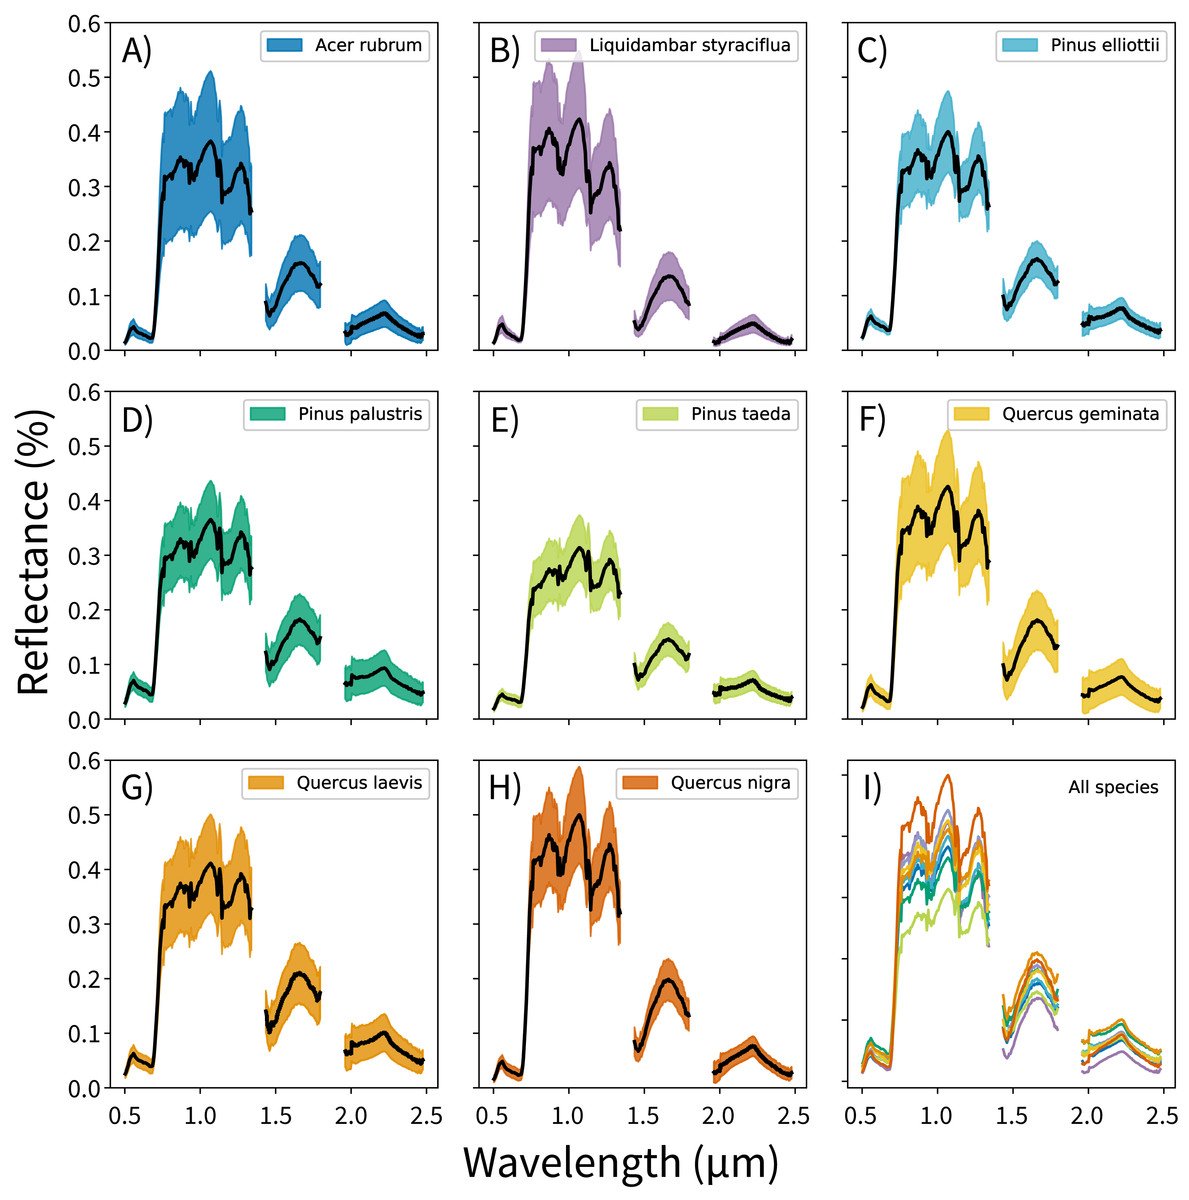
\includegraphics[width=\textwidth]{ch2-spectra}
\centering
\caption[Mean reflectance signals showing high interspecific variation for eight target tree species.]{(A-H) Canopy reflectance profiles for eight tree species with mean reflectance values in black and $\pm$ 1 standard deviation in color. (I) Mean reflectance values for all species, with each color corresponding to the individual species panels.}
\label{fig:spectra}
\end{figure}

The input NEON data were ``Spectrometer orthorectified surface directional reflectance–flightline (NEON.DP1. 30008)" products. The canopy reflectance data were preprocessed using two steps: outlier removal and dimensionality reduction. In the outlier removal step, the reflectance data were spectrally subset, transformed using principal components analysis (PCA), then thresholded to isolate spurious values. First, reflectance values from the blue region of the spectrum ($0.38-0.49\, \mu m$) and from noisy bands ($1.35-1.43\, \mu m$, $1.80-1.96\, \mu m$, and $2.48-2.51\, \mu m$) were removed. These bands correspond to wavelengths dominated by atmospheric water vapor, and do not track variations in plant traits \cite{Gao2009-on}. This reduced the data from 426 to 345 spectral bands.

Next, these spectrally-subset samples were transformed using PCA. The output components were whitened to zero mean and unit variance, and outliers were identified using a $3\sigma$ threshold. Samples with values outside of $\pm$ three standard deviations from the means (i.e., which did not fall within 99.7\% of the variation for each component) for the first 20 principal components were excluded from analysis. These samples were expected to contain non-vegetation spectra (e.g., exposed soil), unusually bright or dark spectra, or anomalously noisy spectra \cite{Feret2014-bb}. The outlier-removed reflectance profiles for each species are shown in Fig. \ref{fig:spectra}. Once the outliers were removed, the remaining spectral reflectance samples were transformed using PCA. This was not performed on the already-transformed data from the outlier removal process, but on the outlier-removed, spectrally-subset reflectance data.

PCA transformations are often applied to airborne imaging spectrometer data to handle the high degree of correlation between bands, and these transformations are highly sensitive to input feature variation \cite{Jia1999-sd}. Furthermore, transforming reflectance data into principal components can isolate the variation driven by measurement conditions from variation driven by functional traits. For example, brightness patterns alone can drive a high percentage of the variance in reflectance signals, which has nonlinear effects across the full spectrum, but PCA rotation isolates this variance into a single component. And though trait-based variation drives a small proportion of total reflectance signal, a single trait can be expressed in up to nine orthogonal components \cite{Asner2015-fx}. This is critical for distinguishing between species. After the transformation, the first 100 of 345 possible components were used as feature vectors for the classification models. This threshold was arbitrary; it was set to capture the majority of biologically-relevant components and to exclude the noisy components that explain a very low proportion of signal variance.

\subsection{Class Imbalance}

Class imbalance refers to datasets where the number of samples are not evenly distributed among classes. Imbalanced datasets are common in classification contexts, but can lead to problems if unaddressed. For example, training classification models with imbalanced data can select for models that overpredict common classes when the method of model selection doesn't weight misclassification penalties relative to the proportion that each class appears in the dataset. The ECODSE training data were imbalanced: after outlier removal, these data contained a total of 6,034 samples from nine classes (eight identified species, one “other species” class; Fig. \ref{fig:balance}). The most common species, \textit{Pinus palustris}, contained 4,026 samples (66\% of the samples) and the rarest species, \textit{Liquidambar styraciflua}, contained 62 samples (1\% of the samples).

\begin{figure}[!ht]
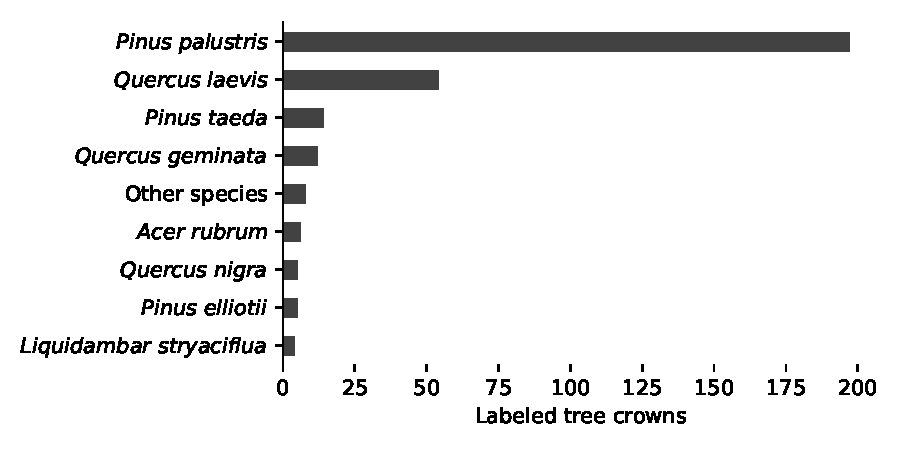
\includegraphics[width=\textwidth]{ch2-balance}
\centering
\caption[Class imbalance in training data based on the number of tree crowns for each species.]{Number of training data crowns for each species. Class imbalance is common in ecology and biogeography, as species abundance distributions typically follow a log series distribution.}
\label{fig:balance}
\end{figure}

These data were resampled prior to analysis to reduce the likelihood of overpredicting common species. Resampling was performed by setting a fixed number of samples per class, then undersampling or oversampling each class to that fixed number. This fixed number was set to 400 samples to split the difference of two orders of magnitude between the rarest and the most common classes. This number was arbitrary, but it was selected to approximate the number of per-species samples recommended in \cite{Baldeck2014-du}. To create the final training data, classes with fewer than 400 samples were oversampled with replacement, and classes with more than 400 samples were undersampled without replacement. The final training data included 400 samples for each of the nine classes (3,600 samples total). Each sample contained a feature vector of the principal components derived from the outlier removed, spectrally subset canopy reflectance data.

\subsection{Model Selection and Probability Calibration}

CCB-ID used two machine learning models: a gradient boosting classifier and a random forest classifier \cite{Friedman2001-nq, Breiman2001-ka}. These models can fit complex, non-linear relationships between response and feature data, can automatically handle interactions between features, and have built-in mechanisms to reduce overfitting \cite{Mascaro2014-et}. They were selected because they perform well in species mapping contexts \cite{Elith2008-ye}, in remote sensing contexts \cite{Pal2005-qh}, and in conjunction with PCA transformations \cite{Rodriguez2006-ha}. Furthermore, these models are built as ensembles of decision trees, resembling the dichotomous key employed by botanists. Unlike a dichotomous key, these models are trained to learn where to split the data since the trait variation that distinguishes species was not known \textit{a priori}.

These models were fit using hyper-parameter tuning and probability calibration procedures. Model hyper-parameters were tuned by selecting the parameters that maximized mean $F1$ scores in fivefold cross-validation using an exhaustive grid search. The $F_1$ score calculates the weighted average of model precision and recall (see \textit{Model evaluation}), and maximizing $F_1$ scores during model tuning reduces the likelihood of selecting hyper-parameters that overpredict common classes and underpredict rare classes. The following parameters were tuned for both models: number of estimators, maximum tree depth, minimum number of samples required to split a node, and minimum node impurity split threshold. The learning rate and node split quality criterion were also tuned for the gradient boosting and random forest classifiers, respectively. All samples were used for hyper-parameter tuning, and the best model hyper-parameters (i.e., the hyper-parameters that maximized mean $F_1$ scores in cross-validation) were used to fit the final models.

Prediction probabilities were calibrated (i.e., adjusted) after the final hyper-parameters were selected, as accurately characterizing prediction probabilities is essential for error propagation and for assessing model reliability. Well-calibrated probabilities should scale linearly with the true rate of misclassification (i.e., model predictions should not be under or overconfident). Some decision tree ensemble methods, such as random forest, tend to be poorly calibrated, however. Since this type of ensemble averages predictions from a set of weak learners—which individually have high misclassification rates but gain predictive power as an ensemble—model variance can skew high probabilities away from one, and low probabilities away from zero. This results in sigmoid-shaped reliability diagrams \cite{DeGroot1983-nc, Niculescu-Mizil2005-nd}.

To reduce these biases, prediction probabilities were calibrated using sigmoid regression for both the gradient boosting and random forest classifiers. The data were first randomly split into three subsets: model training (50\%, or 200 samples per class), probability calibration training (25\%, or 100 samples per class), and probability calibration testing (the remaining 25\%). Each classifier was fit using the model training subset and the tuned hyper-parameters. Prediction probabilities were calibrated with sigmoid regression using the probability training subset, and internal threefold cross-validation to assess the calibration. Calibrated model performance was assessed using the holdout test data. After these assessments, the final models were fit using the model training data, then calibrated using the full probability training and testing data (i.e., the full 50\% of samples not used in initial model training).

\begin{figure}[!ht]
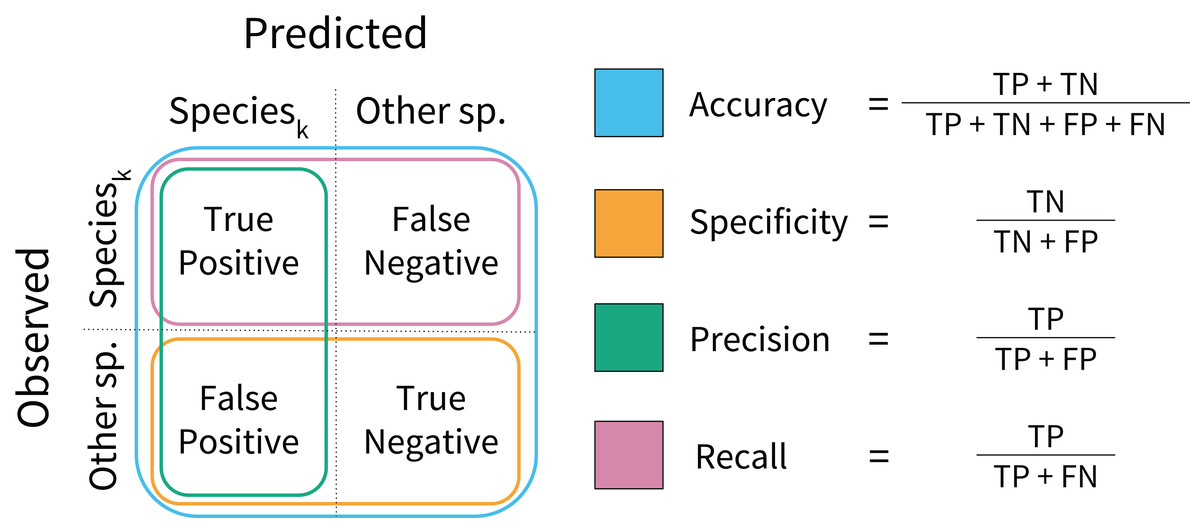
\includegraphics[width=\textwidth]{ch2-metrics.jpg}
\centering
\caption[Summary of the classification model metrics calculated on per-pixel and per-species bases.]{Summary of the classification model metrics calculated on per-pixel and per-species bases. A confusion matrix was computed for each species, and each metric was calculated in a one-vs-all fashion.}
\label{fig:metrics}
\end{figure}

\subsection{Model Evaluation}

During model training, performance was assessed on a per-sample basis using model accuracy and log loss scores. Model accuracy calculates the proportion of correctly classified samples in the test data (Fig. \ref{fig:metrics}), and high model accuracy scores are desirable. Log loss assesses whether the prediction probabilities were well calibrated, penalizing incorrect and uncertain predictions. Low log loss scores indicate that misclassifications occur at rates close to the rates of predicted probabilities. During model testing, performance was assessed using rank-1 accuracy and cross-entropy cost \cite{Marconi2018-wn}. Rank-1 accuracy was calculated based on which species ID was predicted with the highest probability. The cross-entropy score is similar to the log loss function, but was scaled using an indicator function. These can be interpreted in similar ways to accuracy and log loss scores; high rank-1 accuracy and low cross-entropy scores are desirable \cite{Hastie2009-fs}.

Secondary model testing metrics were calculated for each species using the test data. These included model specificity, precision, and recall (Fig. \ref{fig:metrics}). These metrics reveal model behavior that accuracy scores may obscure. Specificity assesses model performance on non-target species, penalizing overprediction of the target species (i.e., a high number of false positives). Precision also penalizes overprediction, but assesses the rate of overprediction relative to the rate of true positive predictions. Recall calculates the proportion of true positive predictions to the total number of positive observations per species. Higher values are desirable for each. These metrics were calculated to aid interpretation, but were not used to formally rank model performance.

Performance during model training was assessed at the sample scale, meaning the model performance metrics were calculated on every pixel (i.e., sample) in the training data. However, the competition evaluation metrics were calculated using crown-scale prediction probabilities, so performance metrics were calculated after aggregating each pixel from individual trees to unique crown identities. To address this scale mismatch, prediction probabilities were first calculated for each sample in a crown using both gradient boosting and random forest models, then the sample-scale probabilities were then averaged by crown.

\subsection{Decomposition Analysis}

Two analyses were performed to assess how PCA transformations affected model performance. Prior to these analyses, I bootstrapped the original model fits to assess model variance. I then compared these bootstrapped fits to models trained with the spectrally-subset reflectance data instead of the PCA transformed data. This was done to evaluate the change in model performance attributed to the PCA rotation. Next, I compared models trained using a varying number of principal components. These models were trained using $n_{pcs}$ $\in$ (10, 20, …, 345) as the input features, with 345 being the maximum number of potential components after spectral subsetting. These comparisons assessed whether the PCA transformations improved model performance and how changing the amount of spectral variation in the feature data affected performance. These were each bootstrapped 50 times to derive an unbiased estimate of the variance in each model.

\section{Results}

\begin{figure}[!ht]
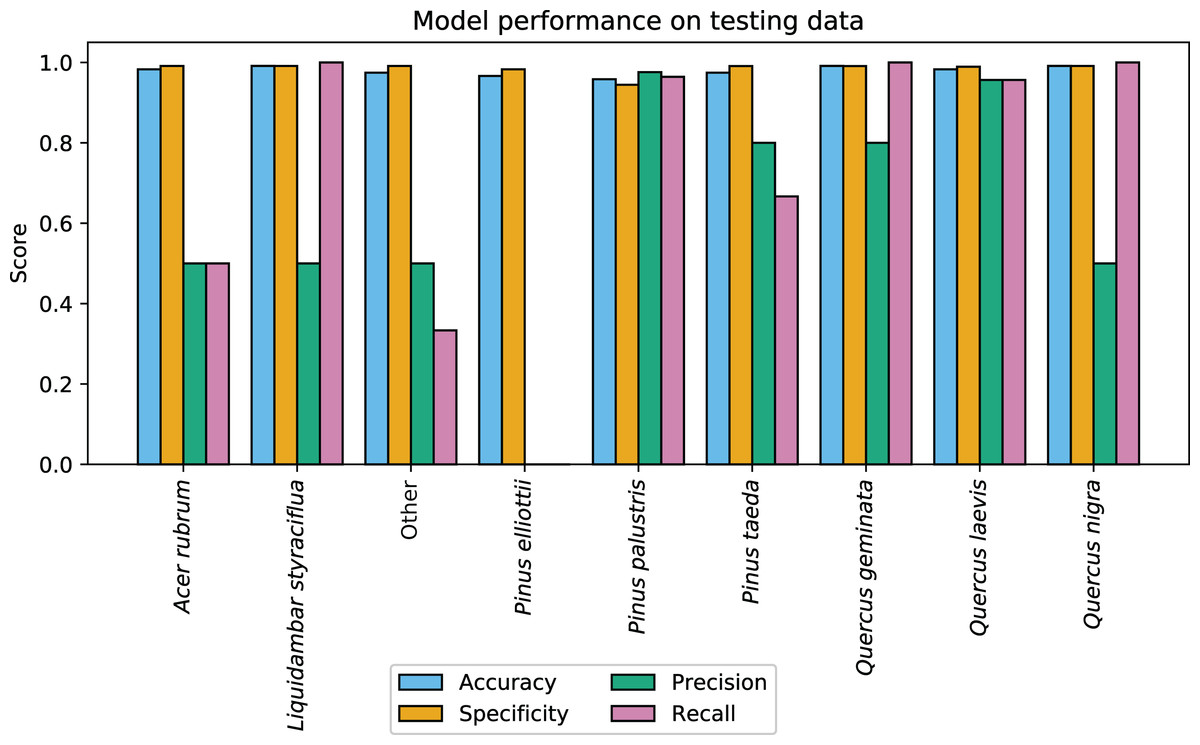
\includegraphics[width=\textwidth]{ch2-performance.jpg}
\centering
\caption[Per-species secondary model performance metrics applied to test data]{Per-species secondary model performance metrics applied to test data, calculated using the binary confusion matrix reported in Fig. \ref{fig:confusion-matrix}. Metrics weighted by the true negative rate (i.e., accuracy and specificity) were high for all species since the models correctly predicted the most common species, \textit{Pinus palustris}. However, metrics weighted by the true positive rate (i.e., precision and recall) were much more variable since there were fewer than six observed crowns for seven of the nine species (\textit{P. palustris} and \textit{Quercus laevis} had 84 and 23 crowns, respectively). This penalized misclassifications of rare species. These metrics were also recalculated using the continuous per-crown prediction probabilities, which can be found in Fig. \ref{fig:performance-continuous}}
\label{fig:performance}
\end{figure}

\begin{figure}[!ht]
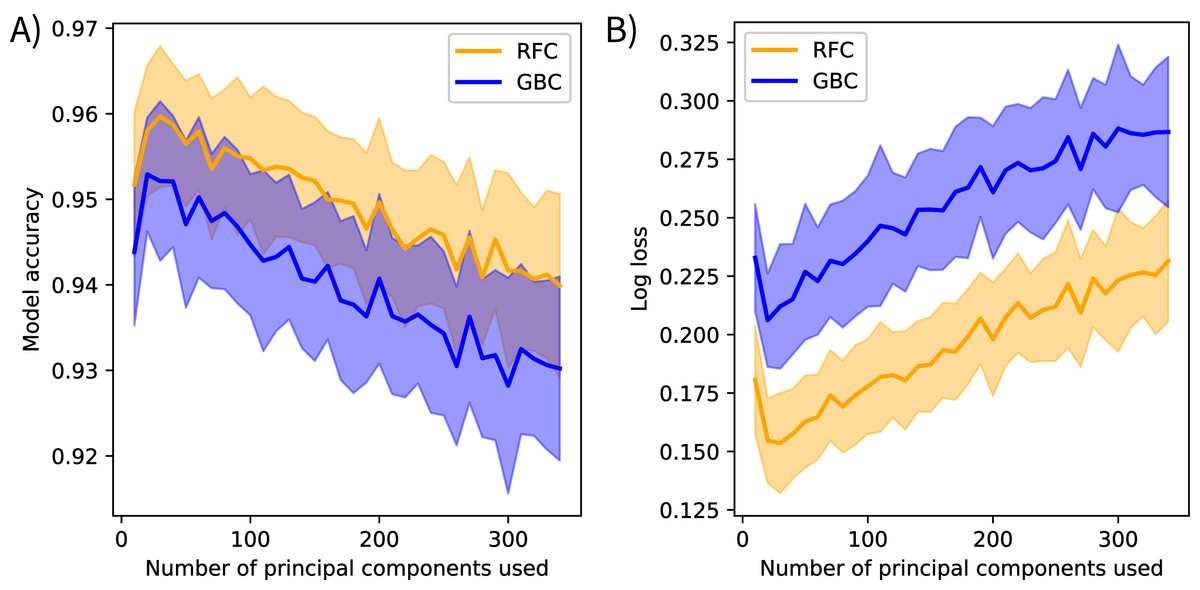
\includegraphics[width=\textwidth]{ch2-pca.jpg}
\centering
\caption[Model accuracy and log loss scores changing as a function of the number in input principal components.]{Mean (solid) and standard deviation (shaded) of (A) model accuracy and (B) log loss scores as a function of increasing spectral variance for each classification method. Scores were calculated on holdout data from the training set, not the competition test data. Using all spectral variance (i.e., all principal components) as model features decreased model performance. Both random forest classifiers (RFC) and gradient boosting classifiers (GBC) were used.}
\label{fig:pca}
\end{figure}

CCB-ID performed well according to the ECODSE competition metrics, receiving a rank-1 accuracy score of 0.919, and a cross-entropy cost score of 0.447 on the test data. These were the highest rank-1 accuracy and the lowest cross-entropy cost scores among participants. Other methods reported rank-1 accuracy scores from 0.688 to 0.88 and cross-entropy scores from 0.877 to 1.448 \cite{Marconi2018-wn}. A confusion matrix with the classification results is reported in Fig. \ref{fig:confusion-matrix}. In addition to the high rank-1 accuracy and low cross-entropy cost scores, the CCB-ID model performed well according to the secondary crown-scale performance metrics. These secondary metrics calculated a mean accuracy score of 0.979, mean specificity score of 0.985, mean precision score of 0.614, and mean recall score of 0.713 across all species. The per-species secondary metrics are summarized in Fig. \ref{fig:performance}. These results were calculated using the categorical classification predictions (i.e., after assigning ones to the species with the highest predicted probability, and zeros to all other species). Probability-based classification metrics are reported in Fig. \ref{fig:performance-continuous}.

During model training, outlier removal excluded 797 samples from analysis. A total of 264 of the 797 samples (33\%) removed from analysis were from \textit{P. palustris}, while the remaining 533 samples (67\%) were from non-\textit{P. palustris} species. Outlier removal disproportionately excluded samples from uncommon species; 45\% of samples from \textit{L. styraciflua}, the rarest species, were removed. After outlier removal, the first principal component contained 78\% of the explained variance. However, this component did not drive model performance; it ranked 7th and 11th in terms of ranked feature importance scores for the gradient boosting and random forest classifiers. Model accuracy scores, calculated on a sample basis (i.e., not by crown) using the 25\% training data holdout, were 0.933 for gradient boosting and 0.956 for random forest. Log loss scores, calculated prior to probability calibration, were 0.19 for gradient boosting, and 0.47 for random forest. After probability calibration, log loss scores were 0.24 for gradient boosting and 0.16 for random forest. The per-class secondary metrics reported a mean specificity score of 0.987, mean precision score of 0.908, and mean recall score of 0.907 across all species.

The post-submission analyses found PCA transformations improved model accuracy. Models fit using the original methods calculated mean bootstrapped accuracy scores of 0.944 ($s.d. \pm 0.009$) for gradient boosting and 0.955 ($s.d. \pm 0.008$) for random forest. Models fit using the spectrally-subset reflectance data as features calculated mean accuracy scores of 0.883 ($s.d. \pm 0.012$) for gradient boosting and 0.877 ($s.d \pm 0.011$) for random forest, and mean log loss scores of 0.46 ($s.d. \pm 0.03$) for gradient boosting and 0.48 ($s.d. \pm 0.03$) for random forest. Mean model accuracies declined and mean log loss scores increased after including more than 20 components as features for the models fit using varying numbers of principal components (Fig. \ref{fig:pca}).

\section{Discussion}

CCB-ID accurately classified tree species using NEON imaging spectroscopy data, reporting the highest rank-1 accuracy score and lowest cross-entropy cost score among ECOSDE participants. These scores compare favorably to other imaging spectroscopy-based species classification efforts, as reviewed by \cite{Fassnacht2016-qb}. These crown-scale test results highlight the technical and conceptual potential of species mapping methods that approximate botanical and taxonomic approaches to classification. However, this method failed to overcome several well-known species mapping challenges, like precisely identifying some rare species. Below I discuss some key takeaways and suggest opportunities to improve future imaging spectroscopy-based species classification approaches.

\subsection{Class Imbalance in Ecological Contexts}

The high per-species accuracy scores indicate a high proportion of correctly classified crowns in the test data. However, accuracy can be a misleading metric in imbalanced contexts. Since seven of the nine classes had six or fewer crowns in the test data (out of 126 total test crowns), classification metrics weighted by the true negative rate (i.e., accuracy and specificity) were expected to be high if the majority class were correctly predicted. Metrics weighted instead by the true positive rate (i.e., precision and recall) showed much higher variation across rare species, as a single misclassification greatly alters these metrics when there are few observed crowns (Fig. \ref{fig:performance}). Due to the small sample size, it is difficult to assess if these patterns portend problems at larger scales. For example, there were two observed \textit{Acer rubrum} crowns in the test data, yet only one was correctly predicted. Was the misclassified crown an anomaly? Or will this low precision persist across the landscape, predicting \textit{A. rubrum} occurrences at half its actual frequency? The latter seems unlikely, in this case; the low cross-entropy and log loss scores suggest misclassified crowns were appropriately uncertain when assigning the wrong label (\ref{fig:performance-continuous}). However, since airborne species mapping is employed to address large-scale ecological patterns where model precision is key (e.g., in biogeography, macroecology, and biogeochemistry), we should be assessing classification performance on more than one or two crowns per species.

Comparing model performance between and within taxonomic groups revealed notable patterns. \textit{Quercus} and \textit{Pinus} individuals (i.e., Oaks and Pines) accounted for 120 of the 126 test crowns and there was high fidelity between them. Only one Quercus crown was misclassified as \textit{Pinus}, and two \textit{Pinus} crowns were misclassified as \textit{Quercus}. From a botanical perspective, this makes sense; these genera exhibit very different growth forms (i.e., different canopy structures and foliar traits), and should thus be easy to distinguish in reflectance data. However, within-genus model performance varied between \textit{Quercus} and \textit{Pinus}. \textit{Quercus} crowns were never misclassified as other \textit{Quercus} species, yet there were several within-\textit{Pinus} misclassifications. 

This may be because \textit{Quercus} species tightly conserve their canopy structures and foliar traits \cite{Cavender-Bares2016-il}, while \textit{Pinus} species may express trait plasticity. \textit{Pinus} species maintain similar growth forms (i.e., their needles grow in whorls bunched through the canopy), perhaps limiting opportunities to distinguish species-specific structural variation. Furthermore, they are distributed across the varying climates of the southern, eastern, and central United States, suggesting some degree of niche plasticity. If this plasticity is expressed in each species’ functional traits, then convergence among species may then preclude trait-based classification efforts. Quantifying the extent to which foliar traits are conserved within and between species and genera will be essential for assessing the potential for imaging spectroscopy to map community composition across large extents \cite{Violle2012-nl, Siefert2015-sk}.

\subsection{Trait-based Interpretations of Imaging Spectroscopy Data}

The post-submission analyses revealed several notable patterns. First, PCA transformation significantly increased mean model accuracy scores by 7-8$\%$ compared to the spectrally-subset reflectance data. I suspect this is because the models could focus on the spectral variation driven by biologically meaningful components instead of searching for that signal in the continuous reflectance spectrum, where the majority of variation is driven by abiotic factors. The low feature importance scores of the first principal component support this interpretation. The first component in reflectance data is typically driven by brightness
—not an indicator of interspecific variation—and contained 78\% of the explained reflectance variance, but ranked low in feature importance for both models. This preprocessing transformation approximates the “rotation forest” approach developed by \cite{Rodriguez2006-ha}, who found PCA preprocessing improved tree-based ensemble models in virtually every context it was applied. They suggested retaining all components to maintain the full dimensionality of the input data. However, the component-based sensitivity analysis showed model accuracy decreased when including more than the first 20 components (Fig. \ref{fig:pca}). Since there are many components that include non-biological information, like brightness or sensor noise, there results suggest that using all components overfits to spurious signals in this feature-rich dataset. Performing feature selection on transformed data will likely help to overcome this. 

Feature selection has been applied to reflectance data to find the spectral features that track functional trait variation \cite{Feilhauer2015-uk}, which should help identify the trait-based principal components that discriminate between species. Furthermore, other transformation methods may be more appropriate than PCA; principal components serve only as proxies for functional traits in this context. I expect transforming reflectance data directly into trait features, further extending the analogy of a taxonomic approach to classification, would improve species mapping accuracy, improve model interpretability, and further define the mechanistic and biophysical basis for species mapping with imaging spectroscopy.

\subsection{Overcompensating for Rarity}

Despite the successes of CCB-ID, there were several missteps in model design and implementation. For example, outlier removal and resampling were employed to reduce class imbalance problems but may instead have exacerbated them. First, the PCA-based outlier removal excluded samples based on deviation from the mean of each component. However, since the transformations were calculated using imbalanced data, the majority of the variance was driven by variation in the most common species. This means outlier removal excluded samples that deviated too far from the mean-centered variance weighted by \textit{P. palustris}. Indeed, 533 of the 797 samples excluded from analysis (67\%) were from non-\textit{P. palustris} species (which comprised only 37\% of the full dataset). This removed up to 45\% of samples from the rarest species (\textit{L. styraciflua}), reducing the spectral variance these models should be trained to identify. This suggests outlier removal should either be skipped or implemented using other methods (e.g., using spectral mixture analysis to identify samples with high soil or non-photosynthetic vegetation fractions) to reduce imbalance for rare species.

Data resampling further exacerbated class imbalance. By setting the resampling threshold an order of magnitude above the least sampled class, the rarest species were oversampled nearly 10-fold in model training. This oversampling inflated per-class model performance metrics by double-counting (or more) correctly classified samples for oversampled species. These metrics were further inflated as a result of how the train/test data were split. The split was performed after resampling, meaning the train/test data for oversampled species were likely not independent. This invalidated their use as true test data, overestimating performance during model training. This was bad practice. Undersampling the common species was also detrimental. Excluding samples from common species meant the models were exposed to less intraspecific spectral variation during training. This is a key source of variation the models should recognize. Excluding this spectral variation made it more difficult for the models to distinguish inter and intraspecific variation. Assigning sample weights (e.g., proportional to the number of samples per class) and using actually independent holdout data could overcome these issues. 

\section{Conclusion}

Airborne imaging spectrometers can map tree species at crown scales across large areas, and these data are now publicly available through NEON's open data platform. However, there is currently no canonical imaging spectroscopy-based species mapping approach, limiting opportunities to explore key patterns in biogeography. This taxonomic learning approach was developed to address this gap and to further the conversation on best practices for species mapping. CCB-ID performed well within the scope of the ECODSE competition, reporting the highest rank-1 accuracy and lowest cross-entropy scores among participants. Yet further testing is necessary to identify whether this method can scale across multiple sites or to other regions, including high diversity forests. I hope CCB-ID will be used by others to improve future species mapping efforts in pursuit of answers to biogeography’s great mysteries of where the species are, and why they are there.

\clearpage